\documentclass[aspectratio=169]{beamer}% only slides

%\documentclass[notes]{beamer}       % print slides + notes
%\documentclass[notes=only]{beamer} % only notes
%\usepackage{pgfpages} %notes
%\pgfpagesuselayout{4 on 1}[a4paper, border shrink=5mm, landscape] %notes
%\usepackage{amsmath}

%\usepackage{callouts}

%\let\note\undefined
\let\note\relax 

\usepackage[text= purple, background = white , arrow = red ]{callouts}
\usepackage{tikz}

%\let\oldcommand\culprit % command from package A causing errors in package B.

%\let\note\relax

%\usepackage{tikz}
%\usetikzlibrary{shapes.callouts}

%\let\note\culprit % command from package A causing errors in package B.


%\usetikzlibrary{shapes.callouts,shadows.blur,positioning,arrows}
%\usepackage[text= gray, background = white , arrow = red ]{callouts}
%\usepackage{tikz}
 %\usepackage{mwe}

%\usetikzlibrary{decorations.text}

\usepackage[french]{babel}

%\usetheme{Boadilla}
\usetheme{Warsaw}
%\usetheme{Madrid}
%\usetheme{Bergen}
%\usetheme{Singapore}
%\usetheme{Antibes}
%\usetheme{Hannover}
%\usecolortheme{crane}
\useinnertheme{rectangles}
%\useoutertheme{tree}
%\usefonttheme{serif}

\usepackage[T1]{fontenc}
\usepackage{uarial}
%\usepackage{multicol}
\addtobeamertemplate{navigation symbols}{}{%
    \usebeamerfont{footline}%
    \usebeamercolor[fg]{footline}%
    \hspace{1em}%
    \insertframenumber/\inserttotalframenumber
}

%\usepackage{multimedia}

\title{Formulaire Web de soumission de projet Sciforma}
\subtitle{Utilisation de l'API REST fournie par Rego Consulting}
\author{Robert Carbonari}
\institute{
\inst{}Direction des ressources informationnelles et des technologies biomédicales\\
CHU Sainte-Justine}
%\institute {CHU Sainte-Justine}
%\institute{Direction des ressources informationnelles et des technologies biomédicales}
%\institute [CHU Sainte-Justine]{\inst{1}Direction des ressources informationnelles et des technologies biomédicales}
\date{\today}

%\beamerdefaultoverlayspecification{<+->}

\begin{document}

\begin{frame}[plain]
\titlepage
%\sound[autostart, inlinesound]{}{paganini.wav}
\end{frame}

\begin{frame}[plain]
%\transduration{5}

%\transblindsvertical
\frametitle{Aperçu}

\tableofcontents
\transwipe 
%\transglitter
\end{frame}

\section{Introduction}
\subsection{L'objectif de cette présentation}
\begin{frame}
Le but de cette présentation est le suivant :
\begin{itemize}[<.->]
\item Présenter un bref historique du projet.
\item Présenter un nouveau formulaire web destiné à remplacer la version papier du formulaire de demande de soumission de projet.
\item Préparer les utilisateurs et les chefs de projet à utiliser le formulaire.
\item Présenter une brève explication de la technologie impliquée pour une meilleure compréhension.

\end{itemize}
\transwipe 
%\transblindsvertical
\end{frame}


\subsection{Contexte}
\begin{frame}
\frametitle{Le contexte}
Début du projet:
\begin{itemize}
	\item En mai 2020, François Charbonneau et Florent Adoubi proposent un projet de création d'un formulaire web pour enregistrer les soumissions de projets dans Sciforma.
	%\note[item]{Le projet consisterait à publier un formulaire Web sur le site intranet du portail hospitalier géré par Kentico qui permettrait aux utilisateurs de la communauté Sainte-Justine de soumettre des propositions de projet destinées à être étudiées pour approbation par le BESP. Après approbation, le projet serait alors automatiquement enregistré dans le système de gestion de projet Sciforma.}
\end{itemize}
\end{frame}

\begin{frame}
\transglitter
\frametitle{Le contexte}
La demande:	
\begin{itemize}%[<.->]
	\item Le formulaire Web devait remplir certaines fonctions de validation.\pause
	\item Les données, une fois validées, devaient être stockées dans une BD pour approbation ultérieure par le personnel de BESP.\pause
	\item Une fois validé et approuvé, le formulaire devait transmettre les données à Sciforma et y créer un nouveau projet.\pause
	\begin{itemize}
		\item Via une API REST fournie par Rego Consulting.\pause
	\end{itemize}
	\item Le système doit envoyer des messages d'accusé de réception automatisés.\pause
	%\note[item]{blah}
\end{itemize}

\end{frame}


\begin{frame}
\transwipe 
\frametitle{Le formulaire actuel au format MS Word}
Voici une partie du document actuel:
\begin{figure}
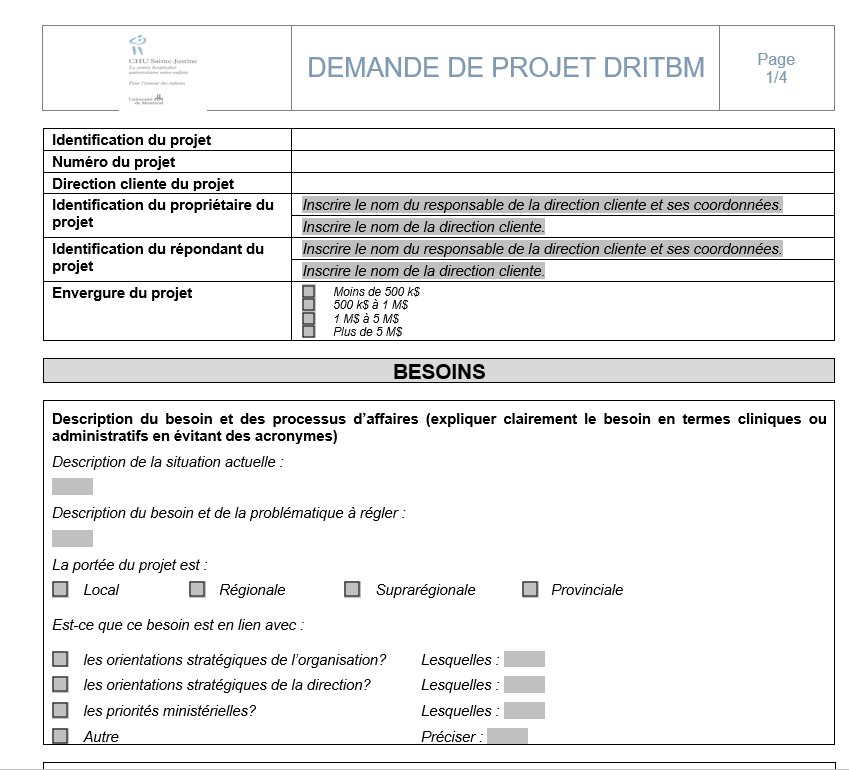
\includegraphics[scale=0.25]{oldForm}
%\caption{Page d'accueil}
\end{figure}
\end{frame}



\subsection{Avantages}
\begin{frame}
\transwipe 
\frametitle{Les avantages}
Avantages de cette approche.:
\begin{itemize}%[<.->]
	\item Avantages en termes de coûts.
		\begin{itemize}
		\item Pas d'achat de licences supplémentaires
		%\note[item]{Étant donné que l'aspect de la saisie des données de Sciforma peut être contrôlé par une application Web, l'institution économise le coût d'achat de licences supplémentaires auprès de Sciforma.}
		\end{itemize}
	\item Avantages d'efficacité.
		\begin{itemize}
		\item Répartition des tâches.
		%\note[item]{La tâche de saisie des données relatives aux soumissions de projets est confiée aux utilisateurs, afin que le personnel de gestion de projet n'ait pas à dupliquer ce travail. Le formulaire Web prend également en charge les tâches de validation et de calcul de base qui seraient normalement laissées aux utilisateurs et aux chefs de projet.}
		\item Validation et calcul automatique des données.
		\end{itemize}
\end{itemize}	
\end{frame}


\subsection{Concept}
\begin{frame}
\transwipe 
\frametitle{Le concept}
\begin{itemize}%[<.->]

	\item Le concept est de créer des demandes de projet dans Sciforma sans avoir besoin d'accéder à l'application en soi.
	\item Collaboration spéciale avec Rego Consulting 
	%\note[item]{ Le mécanisme consiste à envoyer des messages au serveur Sciforma via un service Web développé par Rego Consulting utilisant des protocoles HTTP.}
	%\note[item]{Le site Web est hébergé sur un site intranet de Kentico. Le code est développé dans le langage de programmation C\# et Transact SQL avec une base de données Microsoft SQL Server prise en charge.}
	\item Ainsi, un formulaire web intermédiaire est créé pour saisir toutes les données relatives aux nouvelles demandes de projets qui seront accessibles à l'ensemble de la communauté Sainte-Justine.
\end{itemize}
\end{frame}

%\section{Accès}
%\subsection{Serveur de test }{https://test.chusj.org/FAD/BESP}
%\href{https://test.chusj.org/FAD/BESP}{https://test.chusj.org/FAD/BESP}


\subsection{Serveurs}
\begin{frame}
\transwipe 
\frametitle{Les Serveurs}
\begin{itemize}%[<.->]

\item Serveur de test 
	\begin{itemize}
	\item https://test.chusj.org/FAD/BESP
	\end{itemize}
\item Serveur de production \color{red}(\small {pas encore mis en production})
	\begin{itemize}
	\item https://app.chusj.org/FAD/BESP
	\end{itemize}
\end{itemize}
\end{frame}

\subsection{Caractéristiques du formulaire Web}
\begin{frame}
\transglitter 
\frametitle{Caractéristiques du formulaire Web}
Caractéristiques:
\begin{itemize}
	\item Il valide la saisie des données.\pause
	\item Il calcule automatiquement les données financières.\pause
	\item Il force la synchronisation des données entre le formulaire et la base de données.\pause
	\item Il envoie des messages de confirmation par courrier électronique.\pause
\end{itemize}
\end{frame}

\section{Mise en œuvre}
\subsection{Page d'accueil}

\begin{frame}
\transwipe 
\frametitle{La page d'accueil}

%\begin{figure}
% \centering
%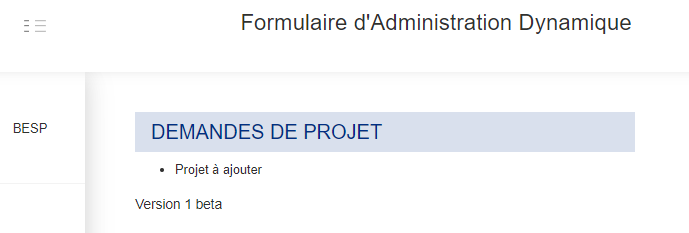
\includegraphics[scale=0.35]{home_everyone}
%%\caption{Page d'accueil}
%\end{figure}
\begin{figure}
    \centering
    \begin{annotate}{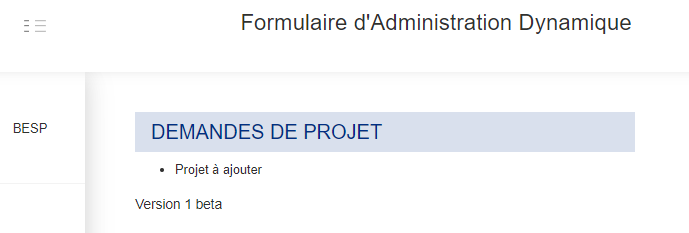
\includegraphics[width=0.35\textwidth]{home_everyone}}{0.35}
        %\helpgrid[gray]
        %\note{6,-0.5}{les utilisateurs réguliers n'ont pas accès à cette option}
        \callout{4,-3}{option visible pour tous les utilisateurs}{-1,-1.25}
%        \arrow{-3,-2.4}{-4.5,-3}
        % And raw tikz
        \draw[very thick,red] (-4,-1.5) rectangle (-1.25,-0.75);
    \end{annotate}
%    \caption{callouts package}
    \label{fig:first}
\end{figure}

\end{frame}

\subsection{Page Demandes De Projet  - liste de demandes}
\begin{frame}
\transwipe 
\label{pictures}
\frametitle{La page d'accueil - liste de demandes}
Voici la page d'accueil - liste de demandes de projets approuvés et non approuvés:

%\begin{figure}
%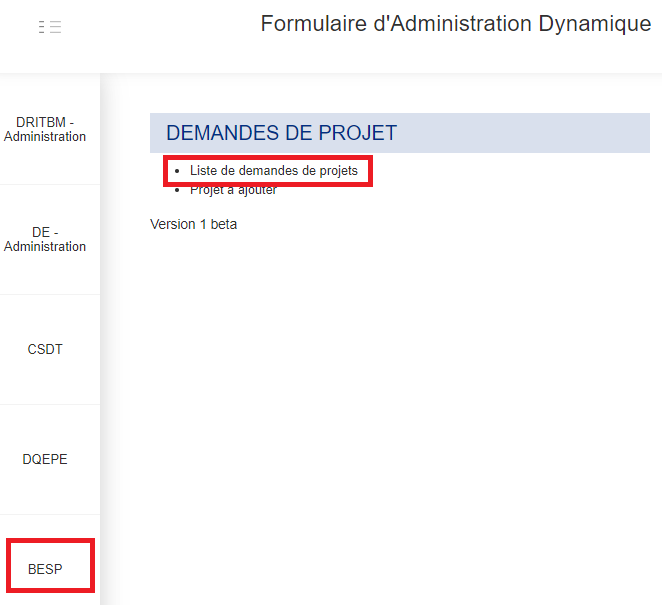
\includegraphics[scale=0.35]{home_list}
%\end{figure}

\begin{figure}
    \centering
    \begin{annotate}{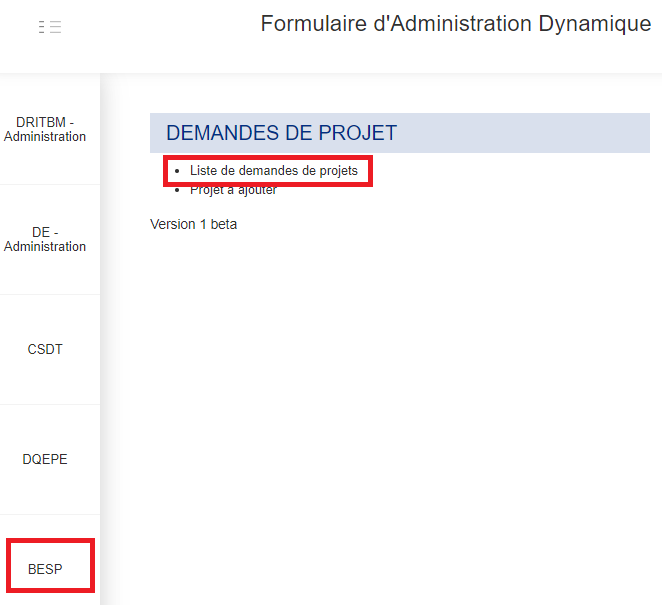
\includegraphics[width=0.35\textwidth]{home_list}}{0.35}
        %\helpgrid[gray]
        \note{6,-0.5}{les utilisateurs réguliers n'ont pas accès à cette option}
        \callout{5,1}{visible uniquement pour les chefs de projet}{1,2.25}
%        \arrow{-3,-2.4}{-4.5,-3}
        % And raw tikz
%        \draw[very thick,red] (-2,-1.5) rectangle (1.5,2.5);
    \end{annotate}
%    \caption{callouts package}
    \label{fig:first}
\end{figure}


%\begin{figure}
%    \begin{annotate}{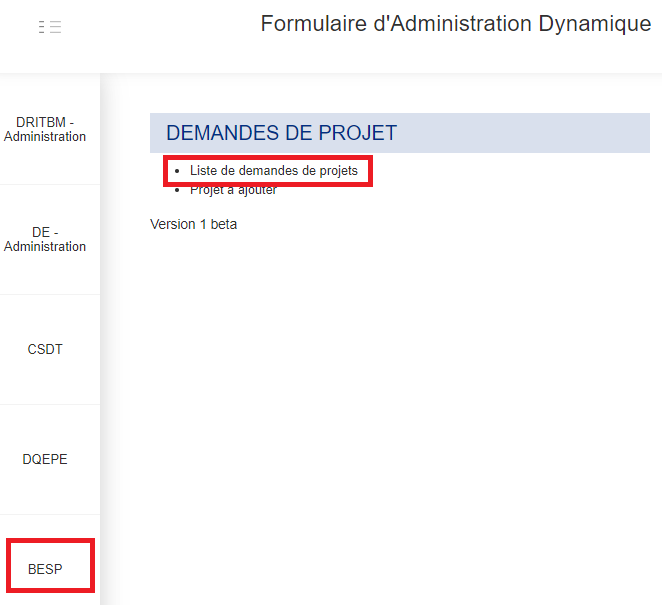
\includegraphics[width=0.35\textwidth]{home_list}}{0.35}
%        \helpgrid[black]
        %\note{3.5,2}{Annotate figures}
%        \callout{3,1}{Butterfly}{1,0.5}
%        \arrow{-3,-2.4}{-4.5,-3}
        % And raw tikz
        %\draw[very thick,red] (-2,-1.5) rectangle (1.5,2.5);
 %  \end{annotate}
%\end{figure}

%\begin{annotate}{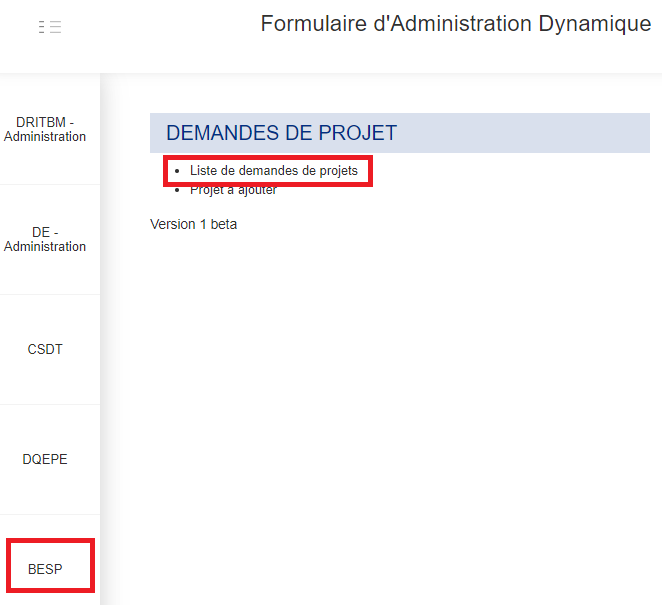
\includegraphics[width=.7\textwidth]{home_list}}{0.25}
% \helpgrid[gray]
% \callout{40,3}{Mushrom}{3,2}
%    \arrow{-3,-2.4}{-4.5,-3}
 %   \end{annotate}


%\begin{annotate}{\ includegraphics[scale=0.35]{home_list}}{0.5}
%\helpgrid
%\end{annotate}

\end{frame}

\subsection{Liste de projets}
\begin{frame}
\transwipe 
\label{pictures}
\frametitle{Liste de projets}

\begin{figure}
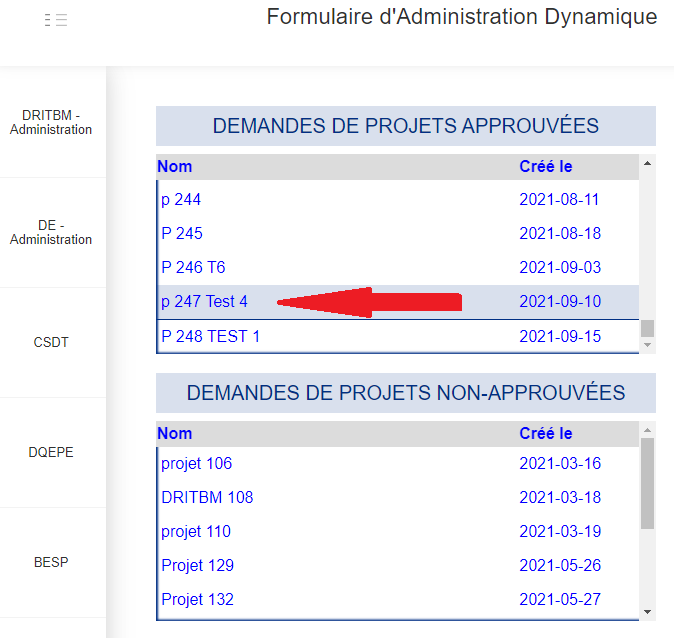
\includegraphics[scale=0.33]{liste_de_demandes}
%\caption{Page d'accueil}
\end{figure}
\end{frame}

\subsection{Demande de projet approuvé}
\begin{frame}
\transwipe 
\label{pictures}
\frametitle{Une demande projet approuvé}

\begin{figure}
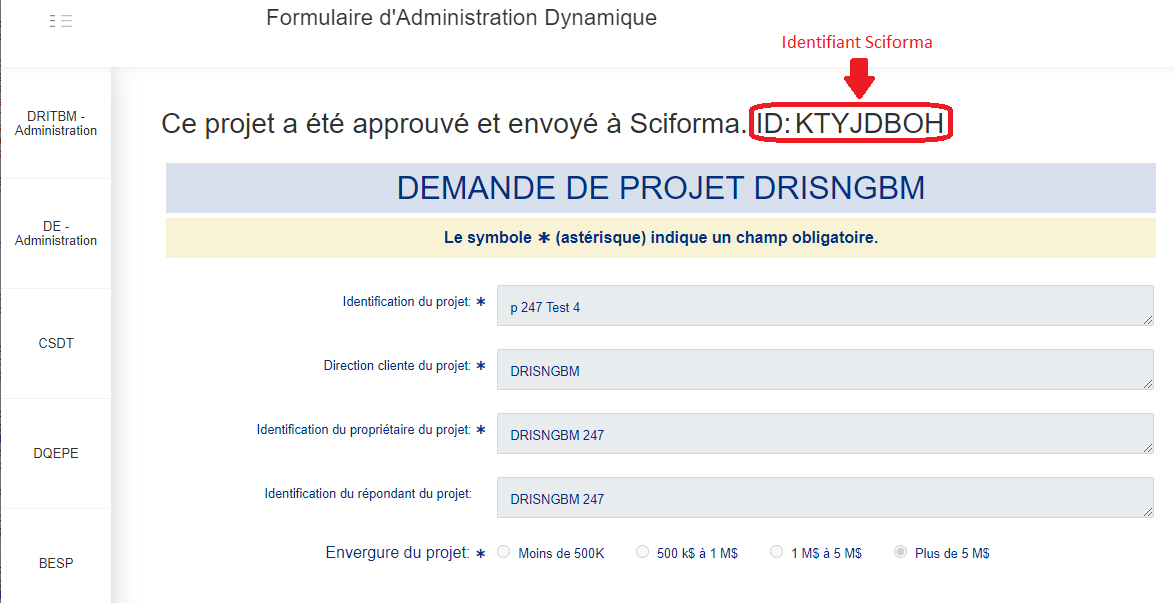
\includegraphics[scale=0.33]{demadeApprouve2}
%\caption{Page d'accueil}
\end{figure}
\end{frame}



\subsection{Page Demandes De Projet - Demande}
\begin{frame}
\transwipe 
\label{pictures}
\frametitle{La page Demandes De Projet - Projet à ajouter}

\begin{figure}
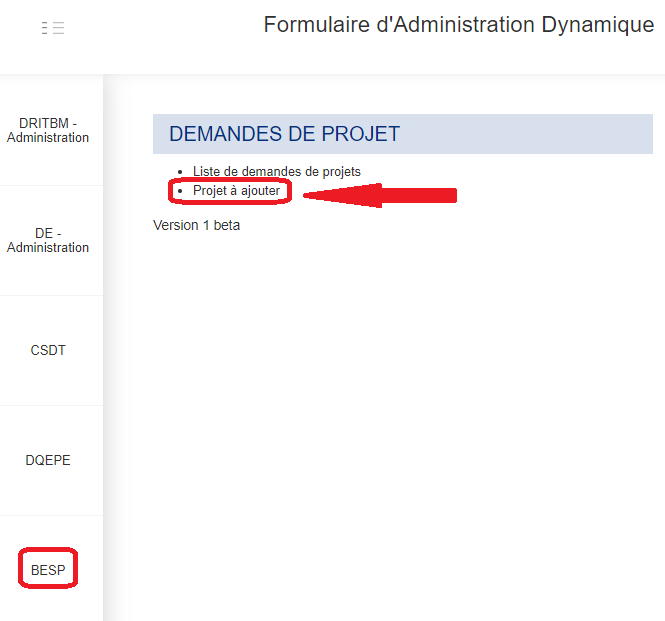
\includegraphics[scale=0.33]{home_list2}
%\caption{Page d'accueil}
\end{figure}
\end{frame}

\begin{frame}
\transwipe 
\label{pictures}
\frametitle{La page Demandes De Projet - Projet à ajouter (suite)}

\begin{figure}
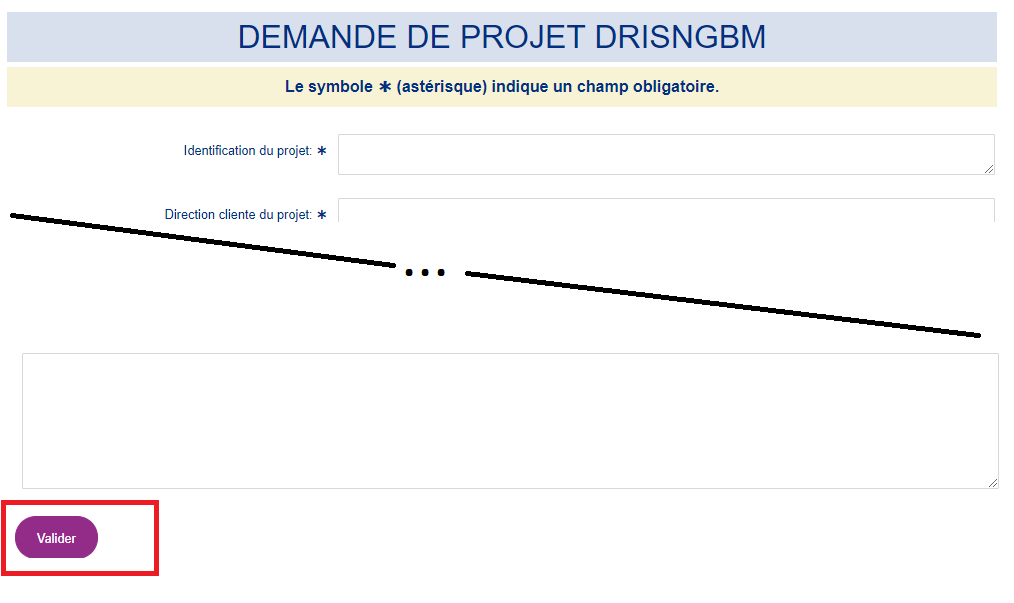
\includegraphics[scale=0.33]{form_valider}
%\caption{Page d'accueil}
\end{figure}
\end{frame}
%---------------------------
\begin{frame}
\transwipe 
  \centering
      \begin{figure}
    \centering
    \begin{annotate}{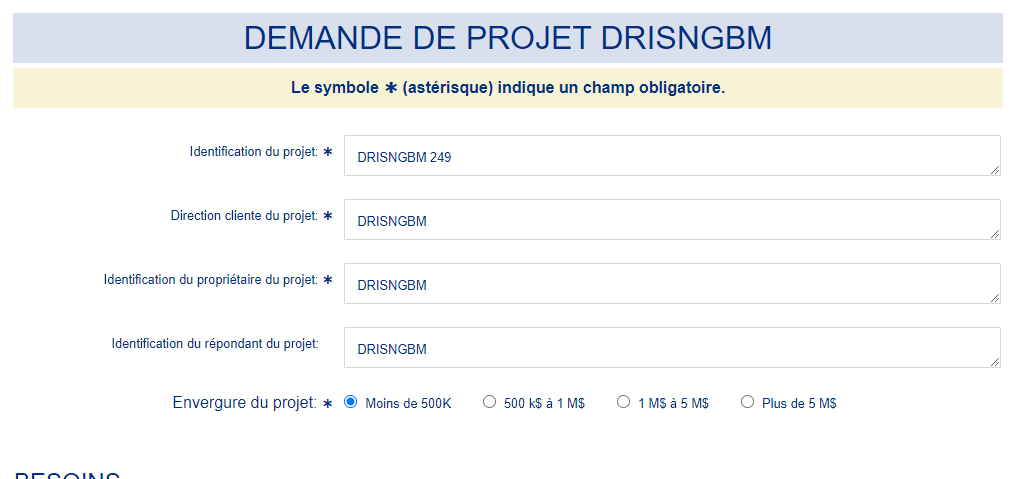
\includegraphics[width=0.75\textwidth]{Projet_a_soumettre}}{0.45}
        %\helpgrid[gray]
        %\note{6,-0.5}{les utilisateurs réguliers n'ont pas accès à cette option}
        \callout{7.5,2}{Titre du nouveau projet qui apparaîtra dans Sciforma}{-1,2}
        %\arrow{-3,-2.4}{-4.5,-3}
        
        \draw[very thick,red] (-1,2.5) rectangle (-4,1.25);
    \end{annotate}
\end{figure}
\end{frame}
    
%++++++++++++++++++++++++++++++++++++++++++++++++++++=
\begin{frame}
\transwipe 
\begin{columns}
\column{0.55\textwidth}
  %===============================
  

    \centering
    \begin{annotate}{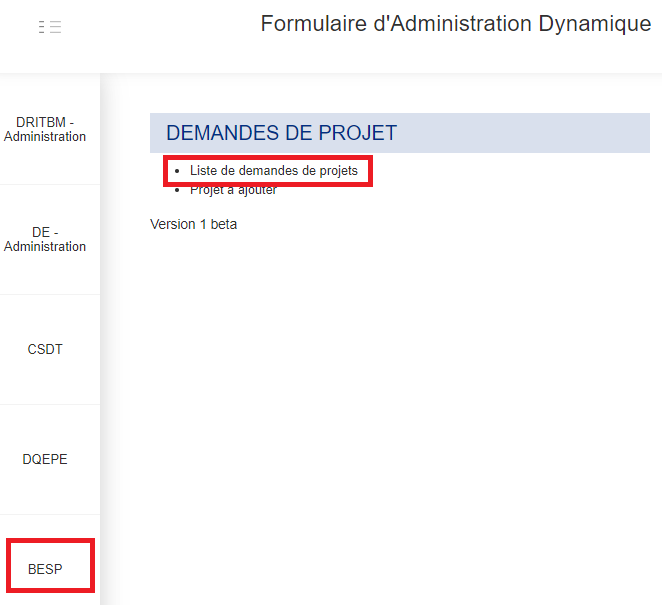
\includegraphics[width=0.85\textwidth]{home_list}}{0.5}
        %\helpgrid[gray]
        %\note{6,-0.5}{les utilisateurs réguliers n'ont pas accès à cette option}
        %\callout{5,1}{visible uniquement pour les chefs de projet}{1,2.25}
        \arrow{1,2.5}{8.5,1}
        % And raw tikz
%        \draw[very thick,red] (-2,-1.5) rectangle (1.5,2.5);
    \end{annotate}
%    \caption{callouts package}
    %\label{fig:first}

  
  %===============================
  \column{0.55\textwidth}

    \centering
    \begin{annotate}{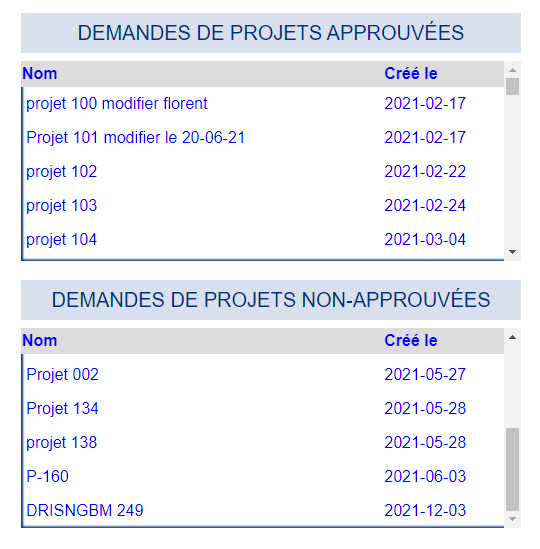
\includegraphics[width=0.85\textwidth]{ Liste-demandes-projets-Nouveau}}{0.35}
       % \helpgrid[gray]
        %\note{6,-0.5}{les utilisateurs réguliers n'ont pas accès à cette option}
        \callout{4,-7}{Projet nouvellement créé}{-4,-8.5}
%        \arrow{-3,-2.4}{-4.5,-3}
        
        \draw[very thick,red] (-4,-9) rectangle (-9,-7.75);
       
    \end{annotate}
    \end{columns}   

\end{frame}
%+++++++++++++++++++++++++++++++++++++++++++++

%Projet_a_soumettre-envoy
\begin{frame}
\transwipe 
\frametitle{Soumission de projet et email de confirmation}
\begin{columns}
\column{0.55\textwidth}
 \begin{annotate}{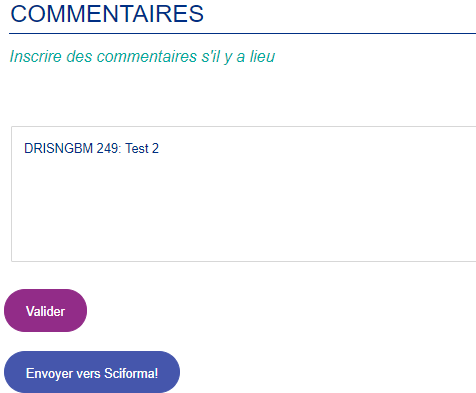
\includegraphics[width=0.85\textwidth]{ Projet_a_soumettre-envoy}}{0.35}
       %\helpgrid[gray]
        %\note{6,-0.5}{les utilisateurs réguliers n'ont pas accès à cette option}
        \callout{4,-7}{chefs de projet uniquement}{-2,-7}
        \arrow{-2.25,-6}{13.5,-3}
        
        \draw[very thick,red] (-2.25,-8) rectangle (-9.25,-6);
       
    \end{annotate}
\column{0.55\textwidth}
%Voici un exemple d'e-mail de confirmation reçu après une nouvelle soumission d'une demande de projet:
\begin{figure}
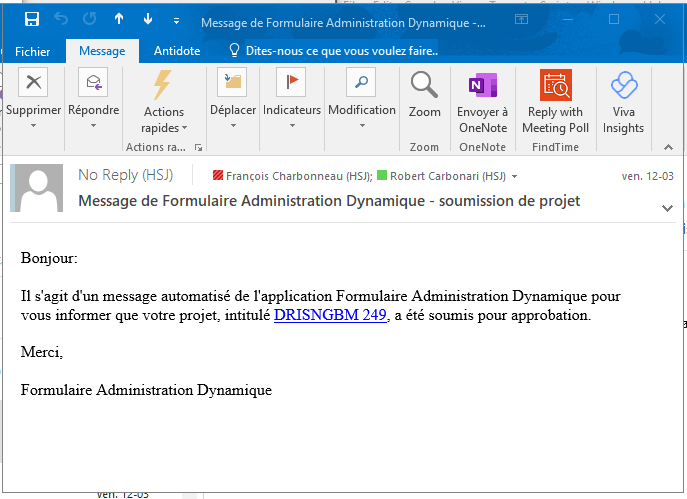
\includegraphics[scale=0.35]{emailConfResubmissionMsg}
%\caption{Page d'accueil}
\end{figure}
 \end{columns}   
\end{frame}

\section{Demo}
\begin{frame}
\transwipe 
%\label{pictures}
\frametitle{Demonstration}
\centering
Faisons une pause pour une démonstration...
%\begin{figure}
%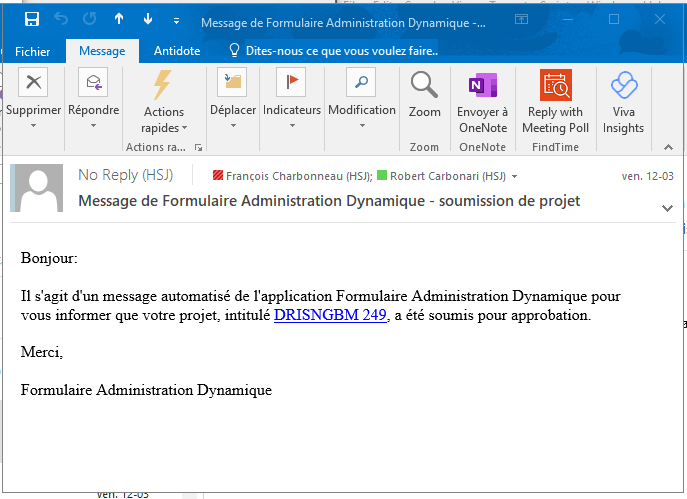
\includegraphics[scale=0.35]{emailConfResubmissionMsg}
%%\caption{Page d'accueil}
%\end{figure}
\end{frame}


\section{Remerciements}
\begin{frame}
\transwipe 
\frametitle{Remerciements}
Je tiens à remercier Patrick Desmarais, dont l'inspiration et la contribution ont rendu cette présentation possible.

\end{frame}


\end{document}